\section{Finite Element Modeling}

All fitness evaluations in the project are based on conclusions drawn from a finite element model. Each design and load case each are represented as slight modifications to a basic model file containing the fixed geometry and ``starting" parameters for the design and loading variables.  \todo{Do I need to summarize the basics of finite element modeling?}

This study makes exclusive use of quadrilaterial shell elements, known to NASTRAN as \codeword{CQUAD4} elements. These elements are 2-dimensional, but do model deformation in all thee dimensions. However, an important assumption made by using these elements is that the entire thickness of the plate distributes the stress applied to the element equally. This implies that deformations in the thickness direction cannot be modeled this way. For example, if a plate can buckle or bend through its thickness this type of element would not be suitable. This model makes use of these elements for the beam flanges, but the elements are oriented to be coplanar with the beam web. This means the flange width is modeled as plate thickness. This orientation will not detect local flange effects such as buckling or local bending. However, this study is primarily concerned with failure of the gross section. Due to the system geometry, these stresses are negligable and therefore the model's inability to properly model them does not appreciably affect the accuracy of this model. This modeling strategy also has the advantage of simplifying the alteration of the flange thickness programmatically. 

\subsection{Selected Model}

\begin{figure}
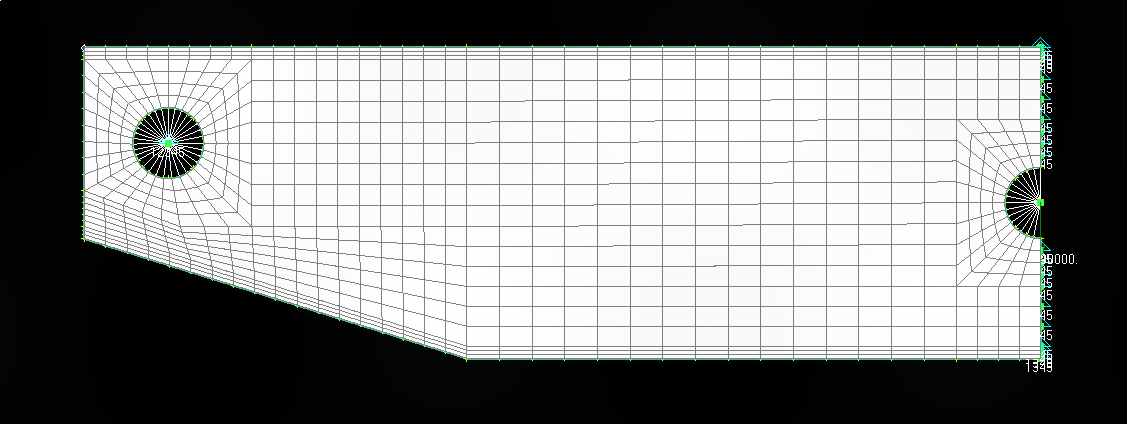
\includegraphics[width=\textwidth]{img/mesh_geom.png}
\label{img:mesh_geom}
\caption{Mesh Geometry as shown in Siemens Femap}
\end{figure}
